% !TeX root = ./main.tex

We now experimentally validate the the performance of the different versions of our algorithms.
Our benchmarks were ran on the VUB Hydra cluster. Each solver call was assigned a single core on a 10-core INTEL Xeon Gold 61482 (Skylake) processor, a timelimit of 120 minutes and a memory-limit of 4GB.
 All code was implemented in Python on top of %CPpy~\footnote{} and
PySAT.\footnote{\url{https://pysathq.github.io}} The MIP solver used is Gurobi 9.0 and when a (Max)SAT solver is used it is RC2 as bundled with PySAT. Within PySAT, the deletion-based MUS extractor MUSX is used as a baseline for comparison.


All of our experiments were ran on a direct translation to CPPY of the \todo{10} puzzles of \citet{ecai/BogaertsGCG20}.\footnote{In one of the puzzles, an error in the automatic translation of the natural language constraints was found and fixed. Because if this error, it was missing in experimental results of the previous work.} 
In all puzzles, we used a cost of 50--70 for using constraints (50 for builtins; 70 for clues) and 1 for previously derived facts. \todo{correct?}

Our experiments were designed to answer the following research questions: 
\begin{compactdesc}
 \item[Q1] What is the effect of requiring optimality of the generated MUSs on the \textbf{quality} of the generated explanations?
 \item[Q2] Which \textbf{domain-specific \grow methods} perform best?
 \item[Q3] What is the effect of the use of \textbf{contrainedness} on the time required to compute an explanation sequence?
 \item[Q4] Does \textbf{re-use} of computed satisfiable subsets improve efficiency?
\end{compactdesc}
In the experiments, more specifically when generating explanation sequence of puzzles, the constraint(s) in the unsatisfiable represent using either \textit{bijectivity}, \textit{transitivity} or \textit{clues} or any combination thereof.

\begin{figure}[ht]
  \centering
  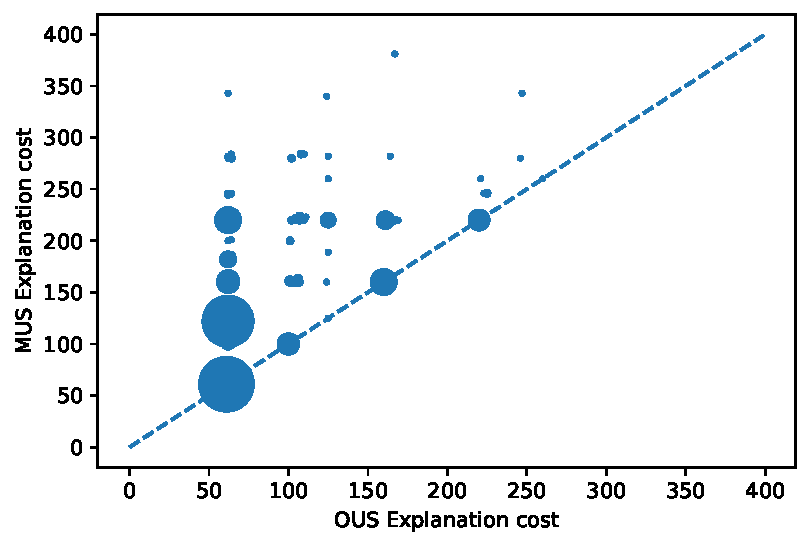
\includegraphics[width=\columnwidth]{figures/rq1.pdf}
  \caption{Q1 - Optimal vs Greedy explanation generation quality}
  \label{fig:rq1}
\end{figure}


\bart{ik schrijf stukje over MUS ECAI}


\paragraph{Explanation quality} 
\bart{Zou een heat map niet beter zijn dan van die dots met size die dan overlappen en het verhaal onduidelijk maken??? } 
To evaluate the effect of optimality on the quality of the generated explanations, we reimplemented a MUS-based explanation generator based on \cref{alg:oneStep}. 
Before presenting the results, we want to stress that this is \emph{not} a fair comparison with the implementation of \citet{ecai/BogaertsGCG20}, since they --- in order to avoid the quality problems we will illustrate below --- implemented an extra inner loop with \emph{even more} calls to \call{MUS} for a selected set fo subsets of \formulac of increasing size (this is their Algorithm~3). 
While this yields better explanations, it comes at the expense of computation time, there leading to several hours to generate the explanation of a single puzzle. 
We will see in our later experiments is that we can \emph{outperform}, in terms of computational cost, a this simple \call{MUS} based implementation while still guaranteeing optimality. \bart{make pareto improvement explict?}

To answer \textbf{Q1}, we ran this \call{MUS}-based as described in \cref{alg:oneStep} and compared at every step the cost of the produced explanation with the cost of the optimal explanation. 
% 
% Similar to \citet{ecai/BogaertsGCG20}, a weight assigned to each type of constraint used. The weighted sum of the constraints present in the 
% (\textit{minimum} / \textit{optimal}) 
% minimal/optimal
% unsatisfiable subset become a proxy to how difficult the generated explanation really is.
% commaring the explanation quality of mus and ous
% To answer \textbf{Q1}, we start by generating a sequence of explanations using the \comus from an initial assignment $I_0$.. Then, using this sequence as a starting point, we look for a MUS-based explanation given the partial assignments $I_i$ at step i.
These costs are plotted in Figure \ref{fig:rq1}, the size of the dot represents the number of occurrences of the combination at hand. 
% Note that, the distribution of the dotts show the quality of the OUS explanation is either similar, when along the same-cost diagonal or better in the upper part of the graph. The dotts' sizes demonstrates 
We see that the difference in quality is striking in many cases, with the MUS-based solution often missing extremely simple explanations (as seen by the large vertical line around cost 50), thereby confirming  
the need for \omus/\comus approach.
\begin{table}[ht]
  \centering
  \begin{tabular}{r||c|c|c|c|c}
    % \begin{tabular}{|r||c|c|c|c|c|c|}
      % \hline
      \textbf{p} & \textbf{MUS} & \textbf{OUS}  & \textbf{OUS+I} & \textbf{\comus} & \textbf{\comus+I} \\
      \hline
      1 &       569 &         4114 &     4727 &           803 &         \textbf{299} \\
      2 &       438 &         3834 &     3972 &           607 &         \textbf{238} \\
      3 &       477 &         4220 &     4938 &           932 &         \textbf{607} \\
      4 &       624 &         3508 &     4820 &           388 &          \textbf{97} \\
      5 &      3382 &         Timeout &     Timeout &          3556 &        \textbf{1537} \\
      6 &       568 &         3849 &     3854 &           498 &         \textbf{155} \\
      7 &       372 &         4411 &     4380 &           685 &         \textbf{414} \\
      8 &       474 &         4679 &     5552 &           669 &         \textbf{448} \\
      9 &       766 &         Timeout &     Timeout &          2383 &        \textbf{1135} \\
      p &       224 &         2601 &     2528 &           651 &         \textbf{537} \\
      % \hline
    \end{tabular}
    \caption{Computation time (s) compared between executions}
    \label{table:computationTime}
  \end{table}

To answer \textbf{Q2} and \textbf{Q3}, we depict the total runtime of different configurations in Table \ref{table:computationTime}: p is the puzzle name\footnote{following the naming of the puzzles introduced in \citet{ecai/BogaertsGCG20}}, 
\emilio{MUS : something ?},
\emph{OUS} algorithm \ref{alg:oneStep} from \citet{ecai/BogaertsGCG20} where the MUS call is replaced by the \emph{OUS} solver.
We compare the following enhancements options to the basic \emph{OUS} algorithm: incrementality by reusing satisfiable subsets between \omus calls (+I), constrainedness in the search for explanations (C).


\paragraph{Computation Time} The naïve \omus approach requires significantly more time to find an optimal MUS. This observation demonstrates that the problem complexity increases when a optimality criterion kicks in. We observe that reusing information throughout the calls to the OUS solver burdens the \onestep algorithm with extra processing in order to keep track of all generated satisfiable subsets.


\paragraph{Constrainedness}
Adding constraindness has two major implications.
First, by guiding the search towards the next cheapest optimal explanation using algorithm \ref{alg:oneStepOCUS}, we effectively reduce the amount of calls to the \omus solver.
The constrainedness enhancement as shown in Table \ref{table:computationTime} proves the importance of our approach.
The explanation generation times for a whole sequence are closer and sometimes even better than the MUS approach even though the problem of finding a OUS is more difficult than finding a MUS.

Second, in practice constrainedness is easily combined with incrementality.
The MIP solver is instantiated only once and is reused across the different \onestep calls of algorithm \ref{alg:oneStepOCUS}.
By keeping the MIP solver warm, we take advantage of its efficiency to handle the many satisfiable subsets which are represented under the form of constraints on the variables of the problem specification.
Table \ref{table:computationTime} demonstrates that contrary to to \emph{OUS+I}, incrementality in \textbf{\comus+I} significantly decreases the overall computation time.

\begin{figure}[ht]
  \centering
  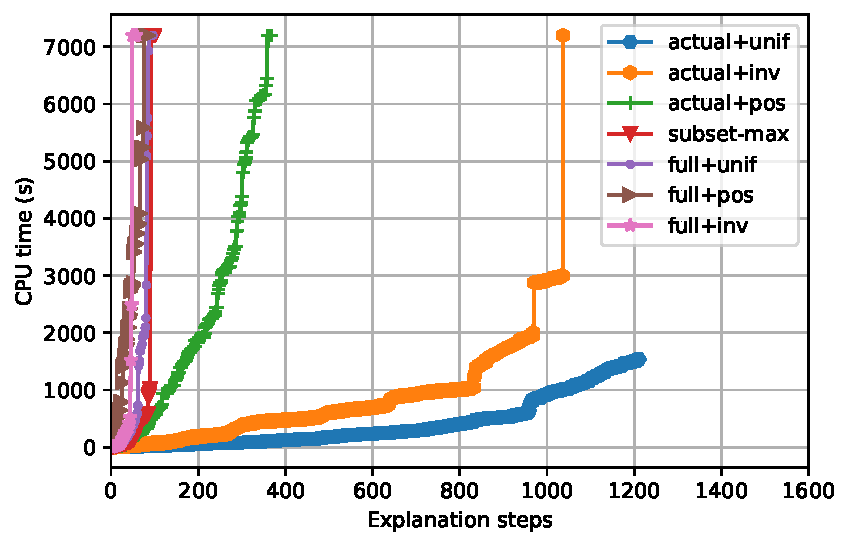
\includegraphics[width=\columnwidth]{figures/rq4.pdf}
  \caption{Q4 - Grow strategies until timeout or full explanation sequence generation}
  \label{fig:rq4}
\end{figure}


\paragraph{Domain-specific \grow} Finally, the core computation of explanations not only lies in the calls to the optimal hitting set solver, but more importantly in computing \emph{high quality} satisfiable subsets.

The latter is reflected in Figure \ref{fig:rq4}.
There are \emilio{some more here!}

% \begin{table*}[]
%     \centering
%     \caption{Execution time generic grow version}
%     \begin{tabular}{|r||c|c|c|c|c|}
%     \hline
%       p &             sat &          subset &      maxsat\_pos &     maxsat\_inv &    maxsat\_unif \\
%     \hline
%      6 &  15.25 - [18]  &  17.46 - [33]  &  48.41 - [9]  &  14.24 - [9]  &  14.71 - [16]  \\
%      8 &  38.95 - [6]  &  21.31 - [10]  &  1558.78 - [6]  &  14.26 - [6]  &  26.47 - [6]  \\
%      p &  14.09 - [9]  &  19.96 - [10]  &  646.94 - [9]  &  6.66 - [1]  &  9.84 - [4]  \\
%      2 &  18.6 - [9]  &  10.12 - [15]  &  171.94 - [9]  &  14.62 - [7]  &  16.54 - [7]  \\
%      7 &  10.24 - [7]  &  17.52 - [8]  &  1542.48 - [1]  &  13.03 - [1]  &  12.31 - [4]  \\
%      1 &  26.25 - [13]  &  20.52 - [13]  &  333.4 - [13]  &  13.28 - [12]  &  16.49 - [13]  \\
%      4 &  40.52 - [101]  &  22.86 - [108]  &  360.07 - [16]  &  14.18 - [11]  &  16.59 - [20]  \\
%      10 &  13.75 - [8]  &  26.72 - [8]  &  487.54 - [2]  &  17.88 - [4]  &  13.89 - [4]  \\
%      3 &  22.58 - [21]  &  19.57 - [10]  &  319.77 - [10]  &  13.49 - [9]  &  14.92 - [9]  \\
%     \hline
%     \end{tabular}
% \end{table*}





\ignore{
We now experimentally validate the the performance of the different versions of our algorithms for explaining satisfiable constraint satisfaction problems.

We consider the following benchmarks: CNF instances from the SATLIB problems Benchmark \cite{hoos2000satlib} and a CNF encoding of the logic grid puzzle ``Origin'' of \cite{ecai/BogaertsGCG20}. All code was implemented in Python on top of %CPpy~\footnote{} and
PySAT.\footnote{\url{https://pysathq.github.io}} The MIP solver used is Gurobi 9.0 and when a (Max)SAT solver is used it is RC2 as bundled with PySAT. Experiments were run on a Intel(R) Xeon(R) CPU E3-1225 with 4 cores and 32 Gb memory, running linux 4.15.0.

Based on the theoretical findings of the previous sections, we aim to answer the following research questions:
\begin{compactdesc}
\item[RQ1] what is the effect of postponing optimal hitting set computation, of incremental OUS solving and of pre-seeding \satsets when solving multiple variants of the same problem?
\item[RQ2] how do the different variants of \omus perform when explaining an elaborate constraint satisfaction problem?
\ignore{
\item[RQ3] how do the sequences found when using (constrained) \omus search compare to those found using a heurisic MUS approach?
}
\end{compactdesc}


\paragraph{RQ1}
To answer the first research question, we use 10 CNF instances from the SATLIB Benchmark and randomly choose 10 literals that are entailed by the CNF. For each variant of the algorithm, we compute the OUS of the same 10 literals in the same order within a total time limit of 10 minutes. 
We compare the following enhancements options to the basic \omus algorithm: postponing optimization (+P), incrementality by reusing satisfiable subsets between \omus calls (+I), and pre-seeding $\satsets$ as described in Section~\ref{sec:incremental} (+W). Options can be combined, for example {\omus}+IPW characterises running the \omus algorithm postponing the optimization phase, with incrementality between the successive calls, and warm starting (pre-seeding) with satisfiable subsets of the original CNF formula.
%The executions are set to timeout after 10 minutes, a limit fixed based on the results of experiment 2.

% \rule{\textwidth}{10pt}

% \begin{table*}[t!]
%     \centering
%     \begin{tabular}{|c|c|c|c|c|c|c|c|c|}
%         \hline
%         % p    & nv& nc&           \omus &      {\omus}+Incr &      {\omus}+Post &  {\omus}+Incr+Warm &   {\omus}+Incr+Post & {\omus}+Incr+Post+Warm \\
%         p    & nv& nc&           \omus &      {\omus}+I &      {\omus}+P &  {\omus}+IW &   {\omus}+IP & {\omus}+IPW \\
%         \hline
%         aim-50-1\_6-yes1-4 & 50& 80&   0.88 s  &   0.38 s  &   0.37 s  &   0.81 s  &    0.65 s  &      \textbf{0.33} s  \\
%         par8-2 & 350 & 1157 &   122.42 s  &  94.07 s  &  96.84 s  &  120.55 s  &  126.15 s  &     \textbf{87.31} s  \\
%         zebra\_v155\_c1135 & 155& 1135&   130.38 s  &  87.97 s  &  84.75 s  &  104.7 s  &  124.48 s  &     \textbf{80.92 s}  \\
%         \hline
%         \end{tabular}
%         \caption{Execution time of the \omus variants for deriving 10 literals evaluated on CNF instances.}
%         \label{table:experiment1}
% \end{table*}

% \begin{table*}[t!]
%     \centering
%     \begin{tabular}{|c|c|c|c|c|c|c|c|c|}
%         \hline
%         % p    & nv& nc&           \omus &      {\omus}+Incr &      {\omus}+Post &  {\omus}+Incr+Warm &   {\omus}+Incr+Post & {\omus}+Incr+Post+Warm \\
%         p    & nv& nc&           \omus &      {\omus}+I &      {\omus}+P &  {\omus}+IW &   {\omus}+IP & {\omus}+IPW \\
%         \hline
%         % 1 & 50& 80&   0.88 s  &   0.38 s  &   0.37 s  &   0.81 s  &    0.65 s  &      \textbf{0.33} s  \\
%         % 2 & 350 & 1157 &   122.42 s  &  94.07 s  &  96.84 s  &  120.55 s  &  126.15 s  &     \textbf{87.31} s  \\
%         % 3 & 155& 1135&   130.38 s  &  87.97 s  &  84.75 s  &  104.7 s  &  124.48 s  &     \textbf{80.92 s}  \\
%         par8-5  & 350  & 1171&      --- &     --- &     --- &     --- &      --- &        --- \\
%         par16-1 & 317 & 1264           &      --- &  --- &  --- &     --- &      --- &     --- \\
%         par16-2& 349 & 1392         &      --- &     --- &     --- &     --- &      --- &        --- \\
%         par16-3 & 334 & 1332        &      --- &     --- &     --- &     --- &      --- &        --- \\
%         par16-4-c & 324 & 1292        &      --- &     --- &     --- &     --- &      --- &        --- \\
%         par16-4  & 1015 & 3324        &      --- &     --- &     --- &     --- &      --- &        --- \\
%         hanoi4  & 718 & 4934       &      1 &     1 &     1 &     1 &      1 &        1 \\
%         \hline
%         \end{tabular}
%         \caption{Number of decision variables explained by the variants of the \omus for timed-out CNF instances.}
%         \label{table:experiment1}
% \end{table*}

% \begin{table*}[t!]
%     \centering
%     \begin{tabular}{c|cccc|cccccc}
%         % \hline
%         p &  time [s] &  \#steps &   $\overline{cost}$ & max(cost) &    1 bij &  1trans &  1 clue & 1 clue+i & 1 mult-i & mult-c. \\
%         \hline
%         1 &  1287.27 &     115 &     25.87  &    25.87  &  31.83\% &  50.57\% &  1.09\% &    16.52 \% &     0\% &    0.0\% \\
%         % \hline
%         \end{tabular}
%         \caption{Puzzle Properties, execution statistics and explanation sequence composition for the origin puzzle.}
%         \label{table:experiment3}
% \end{table*}

% ------------------------------- EMILIO LOCK -----------------------------------------
The results can be seen in Table \ref{table:experiment1} and can be summarized as follows: p, nv and nc represent the instance name, the number of variables and the number of clauses respectively. 
Only for instances aim-50-1\_6-yes1-4, par8-2.cnf and zebra\_v155\_c1135.cnf, is the algorithm able to complete the search for OUSs on the 10 decision variables within the required time constraint of 10 minutes.
For these instances, the overall winner is \emph{{\omus}+IPW}. 
All variants time out on the larger instances (par8-5, par16-1, par16-2, par16-3, par16-4-c, par16-4, hanoi4) before finding the OUSs for all 10 decision variables. For instance par8-5, all variants are able to find 6 out of the 10 variables. On all instances that timed-out, \emph{{\omus}+IPW} remains the fastest. Similar results are observed for the remaining instances for all variants par16-* and hanoi4 with the \omus found for only 1 variable.


A further analysis of the overall execution times highlights that much time is spent in the grow procedure, for which we start from the partial assignment found by the SAT check and use the RC2 MaxSAT solver to complete it. 
We reran the same experiments with a greedy grow algorithm instead and observed that \omus is not even able to finish for zebra\_v155\_c1135 and all runtimes increase considerably.
Furthermore, we see that in this case postponing the MIP call effectively redistributes 50\% of the computational load to growing \satsets and the remaining 50 \% are evenly distributed between (i) the SAT solver, (ii) the MIP solver, and (iii) the the greedy and incremental hitting set heuristics. Hence, while the portion of time spent growing satisfiable subsets is reduced, much more iterations are needed to find the optimal OUSs. %runtime of grow is decreased, the number of 
% A further analysis of the overall execution times highlights that the main bottleneck of the algorithm is the time spent WE NEED TEXT HERE AFTER TEH RUNS ARE READY\todo{emilio}

From this experiment we conclude that in the short time limit provided, the best configuration for computing multiple related OUS's is \emph{{\omus}+IPW}, taking advantage of the repeated calls to the OUS algorithm, thus reusing the computed \satsets.
% ------------------------------- EMILIO LOCK -----------------------------------------

% \begin{table*}[h!]
%     \begin{tabular}{|c|c|c|c|c|c|c|c|c|}
%         \hline
%         % p    & nv& nc&           \omus &      {\omus}+Incr &      {\omus}+Post &  {\omus}+Incr+Warm &   {\omus}+Incr+Post & {\omus}+Incr+Post+Warm \\
%         p    & nv& nc&           \omus &      {\omus}+I &      {\omus}+P &  {\omus}+IW &   {\omus}+IP & {\omus}+IPW \\
%         \hline
%         1 & 50& 80&   0.88 s  &   0.38 s  &   0.27 s  &   0.81 s  &    0.65 s  &      0.33 s  \\
%         2 & 350 & 1157 &   22.42 s  &  14.07 s  &  76.84 s  &  20.55 s  &  126.15 s  &     87.31 s  \\
%         3 & 155& 1135&   130.38 s  &  87.97 s  &  64.75 s  &  104.7 s  &  124.48 s  &     80.92 s  \\
%         4..10 & x $\cdot$ $10^2$ & x $\cdot$ $10^3$           &      --- &     --- &   --- &  --- &   --- &     --- \\
%         % 5 & 317 & 1264           &      --- &  --- &  --- &     --- &      --- &     --- \\
%         % 6 & 324 & 1292        &      --- &     --- &     --- &     --- &      --- &        --- \\
%         % 7 & 334 & 1332        &      --- &     --- &     --- &     --- &      --- &        --- \\
%         % 8& 349 & 1392         &      --- &     --- &     --- &     --- &      --- &        --- \\
%         % 9  & 1015 & 3324        &      --- &     --- &     --- &     --- &      --- &        --- \\
%         % 10  & 718 & 4934       &      --- &     --- &     --- &     --- &      --- &        --- \\
%         \hline
%         \end{tabular}
%         \caption{Comparison of \omus variants evaluated on CNF instances.}
%         \label{table:experiment1}
% \end{table*}

% \begin{table*}
%     \begin{tabular}{|c|c|c|c|c|c|c|}
%         \hline
%         p                  &           \omus &      {\omus}+Incr &      {\omus}+Post &  {\omus}+Incr+Warm &   {\omus}+Incr+Post & {\omus}+Incr+Post+Warm \\
%         \hline
%         1 &    0.88 s | 10 &   0.38 s | 10 &   0.27 s | 10 &   0.81 s | 10 &    0.65 s | 10 &      0.33 s | 10 \\
%         2            &   22.42 s | 10 &  14.07 s | 10 &  76.84 s | 10 &  20.55 s | 10 &  126.15 s | 10 &     87.31 s | 10 \\
%         3  &  130.38 s | 10 &  87.97 s | 10 &  64.75 s | 10 &  154.7 s | 10 &  124.48 s | 10 &     80.92 s | 10 \\
%         4            &      600 s | 1 &  600 s | 2 &  600 s | 1 &     600 s | 1 &      600 s | 1 &     600 s | 1 \\
%         5         &      600 s | 1 &     600 s | 1 &     600 s | 1 &     600 s | 1 &      600 s | 1 &        600 s | 1 \\
%         6         &      600 s | 1 &     600 s | 1 &     600 s | 1 &     600 s | 1 &      600 s | 1 &        600 s | 1 \\
%         7         &      600 s | 1 &     600 s | 1 &     600 s | 1 &     600 s | 1 &      600 s | 1 &        600 s | 1 \\
%         8          &      600 s | 6 &     600 s | 6 &     600 s | 2 &     600 s | 6 &      600 s | 2 &        600 s | 2 \\
%         9         &      600 s | 1 &     600 s | 1 &     600 s | 1 &     600 s | 1 &      600 s | 1 &        600 s | 1 \\
%         10            &      600 s | 6 &     600 s | 6 &   600 s | 6 &  600 s | 6 &   600 s | 6 &     600 s | 6 \\
%         \hline
%         \end{tabular}
%         \caption{Comparison of \omus variants evaluated on CNF instances.}
%         \label{table:experiment1}
% \end{table*}


\paragraph{RQ2}
The second research question is: how do the different variants perform when explaining an elaborate constraint satisfaction problem? For this, we tested the complete generation of an explanation sequence. 
In this comparison, we expect that constrained versions of our algorithm perform best as they will allow performing an entire step of the explanations in a single call.
For this reason, we only include different variations on the constrained configuration and the single best variant of non-constrained algorithms found in the previous experiment. 

% \begin{figure}[t]
%     \centering
%     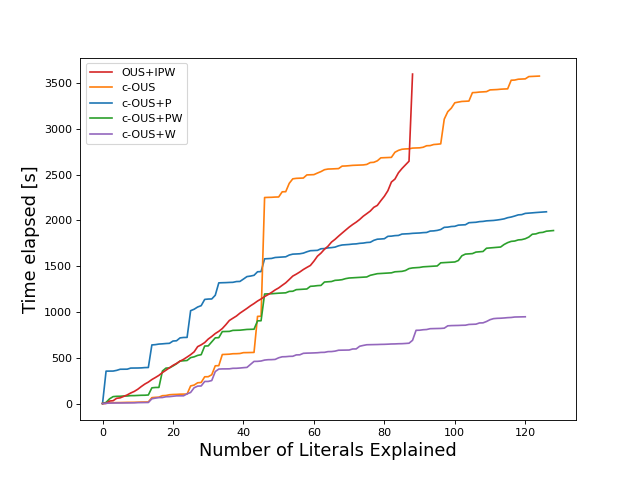
\includegraphics[width=\columnwidth]{figures/omusConstrCumulative.png}
%     \caption{Experiment 2}
%     \label{fig:exp2}
% \end{figure}

We generate the explanation sequence as far as possible within a time limit of one hour. 
The results for the  ``origin'' puzzle is shown in Figure~\ref{fig:exp2}.
It shows the number of literals explained on the X-axis, and the cumulative time taken on the Y-axis. 
Only three configurations find the full explanation sequence (note that there can be multiple optimal sequences with a different length, which explains the difference in length between the configurations).
We  see that the best non-constrained implementation is unable to explain all of the literals within the time limit; especially around step 95 there is a big jump in runtime. The vanilla constrained-OUS approach is not able to finish in time either, with big jumps in time on specific (large and costly) explanation steps.

When combining constrained-OUS with either pre-seeding, post-poned optimisation or both, then our approach is able to fully explain the solution. Best results are obtained with constrained-OUS with just pre-seeding at the beginning. The post-poned optimisation in this case may spent a lot of time generating MCSs that are not or little relevant to the constrained OUSs we are seeking. 

\paragraph{Concluding notes}
While a direct comparison of the runtime needed to find an explanation sequence of our tool versus the one of \citet{ecai/BogaertsGCG20} %built on the IDP system \cite{WarrenBook/DeCatBBD14} 
would shed more light on the performance impact, we can not do a fair comparison as the solvers and hardware used are different.

However, the authors reported that explaining a single puzzle easily takes one to two hours due to the many MUS calls. In contrast, Figure~\ref{fig:exp2} shows that three of our constrained-OMUS approaches fully explain a puzzle one of their larger puzzles in 20 to 30 minutes.
Furthermore, our algorithms guarantee that each explanation step is \emph{optimal} with respect to $f$. As such we know that the generated sequences are at least as good for the cost function provided.

% do not include such an extensive experiment here since it would not be a fair comparison of the underlying algorithms. Indeed, different solving technology is used for finding MUSs, and satisfying assignments. 
%We can, however, give an indication of the speed by mentioning that in some preliminary experiments (e.g., on the origin puzzle), using constrained \omus calls, we can find the entire sequence in roughly 20 minutes, whereas the IDP-based tool takes over two hours.


% Finally, for \textbf{RQ3} \emilio{Bart: concluding phrases on expl. generation}
%  we compare the sequence found by our proposed method with the sequence reported on in~\cite{ecai/BogaertsGCG20} for the origin puzzle (puzzle 1). 
% The explanation sequence for the puzzle is generated using \omus Constr with pre-seeding and according to the same cost function as Bogaerts et al.~\cite{ecai/BogaertsGCG20}. We report statistics relating to the explanation generation in table~\ref{table:experiment3}.
% Evidently, one of the most important observations is the speed-up provided by \omus Constr. 
% As a matter of fact, the sequence is generated in a bit more than 21 minutes compared to a few (2-3) hours in~\cite{ecai/BogaertsGCG20}, meaning that \omus Constr is 8-10x faster, while also finding the optimal explanations in each step.
% Table \ref{table:experiment3} also reports that the explanation sequence has become easier to understand: the average cost is slightly lower and so is $max(cost)$, the cost of the most difficult explanation in the puzzle. 


% \begin{table*}
%     \begin{tabular}{ccc|ccc|cccccc}
%         % \hline
%         types &  $|dom|$ &  $|grid|$ &  time [s] &  \#steps &    cost &    1 bij &  1trans &  1 clue & 1 clue+i & 1 mult-i & mult-c. \\
%         \hline
%         4 &      5 &     150 &  1287.27 &     115 &        25.87 &  27.83\% &  49.57\% &  6.09\% &    11.3\% &     5.22\% &    0.0\% \\
%         % \hline
%         \end{tabular}
%         \caption{Puzzle Properties, execution statistics and explanation sequence composition for the origin puzzle.}
%         \label{table:experiment3}
% \end{table*}

%
%\begin{figure*}[ht]
%    \centering
%    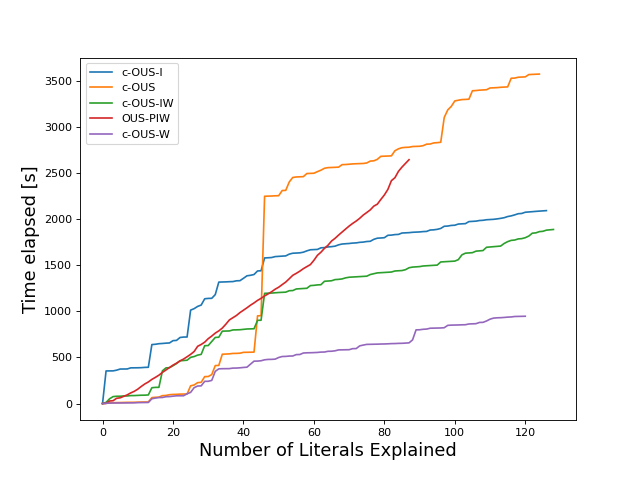
\includegraphics[width=\columnwidth]{figures/omusNonConstrCumulative.png}
%    \caption{}
%    \label{}
%\end{figure*}

% \begin{figure}[ht]
%     \centering
%     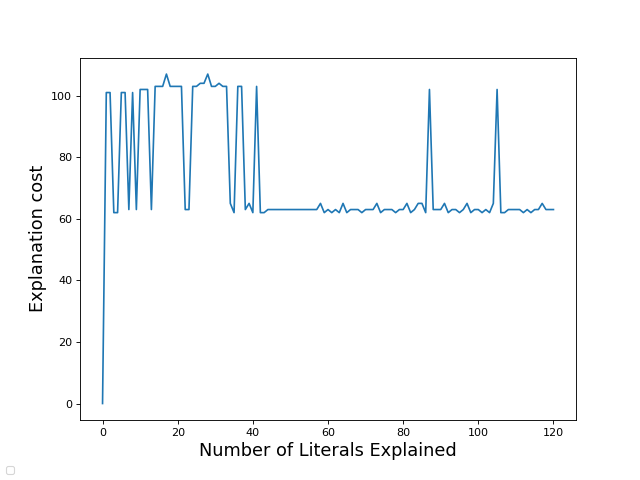
\includegraphics[width=\columnwidth]{figures/explanation_cost.png}
%     \caption{}
%     \label{}
% \end{figure}

}
